\ofsubsection{Maria \& Draco}
%
\ofquote{"O Oeste e o Leste estão travando uma guerra. Draco, o grande herói do Oeste, pensa em sua amada Maria. Estará ela segura? Estará ela me esperando? As forças do Oeste cairam e o castelo de Maria, tomado. O príncipe Ralse, do Leste, tomou a mão dela à força. Mas ela nunca deixou de suspirar pelo Draco..."\\}{Excerto da opera Maria \& Draco}
%
\vfill
%
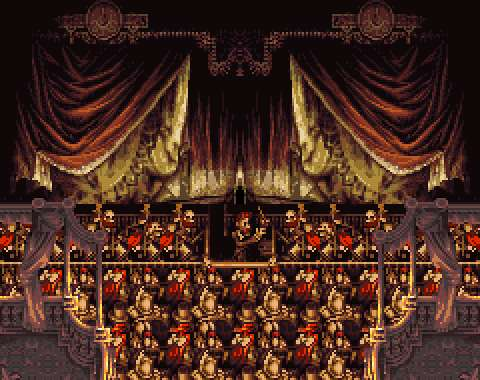
\includegraphics[width=\columnwidth]{./art/mariaanddraco/opera.jpg}
%
\vfill
%
\accf{Maria \& Draco} é uma aventura preparada para ser completada em uma única sessão, projetada para um grupo de personagens de nível 3. 
A história deles devem explicar o porquê de estarem na rica cidade de Jidoor.
Nesta aventura, o grupo é incumbido de evitar o rapto de uma famosa cantora de opera.
%
\vfill
%
\ofquote{"Isto é simplesmente terrível! Quero que a apresentação seja um sucesso, mas não quero que a Maria seja sequestrada!"}{Empresário}
%
\vfill
%
Enquanto descansando na cidade de Jidoor, os aventureiros encontram o proprietário da casa de opera, o auto intitulado "Empresário".
Ele é um homem velho, bem vestido e está constantemente preocupado sobre a próxima opera, "Maria \& Draco".
Ele está desesperado, procurando por guardas de segurança para a apresentação de amanhã e oferece 1.000G para o grupo aceitar o trabalho, o qual aceitam, mesmo não sendo pagos em adiantado.
Na manhã do grande dia, eles encontram o Empresário na casa de opera. Ao entrar, ele está correndo de um lado ao outro freneticamente e ao notá-los, imediatamente lhes entrega a seguinte carta.\\
%
\vfill
%
Querida Maria,\vspace{0.6cm}\\
Decidi tomá-la como esposa, portanto, virei raptá-la.\vspace{0.6cm}\\
\hspace*{0.5cm}O apostador andarilho\\
%
\newpage
%
Após ter se acalmado, o Empresário explica que o "Apostador andarilho" é um homem chamado Setzer Gabbiani e que já lhe causou problemas no passado.
Ele ainda descreve Setzer como "um apostador vagabundo que encontrou sua liberdade além da estreita visão de moralidade da sociedade, à bordo de sua aeronave", em tom sarcástico.
Empresário também explica que Maria é a estrela do show, portanto, sua segurança é de extrema importância.
Ele propõe o seguinte plano para a manter segura: um dos membros do grupo devem representar o papel de Maria e servir de isca.
Ele espera que Setzer aja no fim da primeira cena e tente levá-la para sua aeronave, mas ao capturar a isca, o grupo pode confrontá-lo ao invés. Também sugere que a isca carregue uma corda, dessa forma, ele ou ela pode puxar o resto do grupo para a aeronave, se necessário.
O grupo pode sugerir outras ideias, mas o Empresário rejeitará qualquer uma que possa por a verdadeira Maria em risco.
Se aceitarem o plano dele, eles terão que escolher um dos seus para atuar a parte de Maria na opera, a partir de então o personagem será tratado como "Maria".
%
\vfill
%
\ofquote{"Es...Espere! Eu sou o GENERAL, não uma opera vagabunda!"}{Celes}\\\\
%
O Empresário mostrará o quarto de Maria a eles, onde a "Maria" pode ser vestir e praticar a parte dela.
A "Maria" tem que se parecer igual à original o máximo possível, baixa, de cabelos loiros e um longo vestido branco.
Portanto, o grupo pode ter de comprar um novo vestido e peruca ou ser criativo de alguma maneira, pois precisam convencer o Empresário a cobrir os gastos.
Eles estão livres para explorar a cidade e comprar ou se preparar até a noite. "Maria" deve praticar o seguinte roteiro para sua parte na primeira cena:
%
\vfill
%
Maria entra no palco.\vspace{0.2cm}\\
"Ó, meu herói, estás tão distante. Verei eu, seu sorriso novamente?"\vspace{0.2cm}\\ 
"O amor se vai, assim como a noite dá lugar ao dia. Trata-se apenas de um sonho passageiro."\vspace{0.2cm}\\ 
"Nosso amor resplandece mais do que o sol. Pela eternidade, para mim haverá de ser somente a ti, o meu escolhido."\vspace{0.2cm}\\ 
Maria pega as flores, sobe as escadas até a sacada no topo do castelo, então ergue-as às estrelas.\vspace{0.2cm}\\
"Devemos nos separar agora. Minha vida seguirá, mas o meu coração jamais desistirá de ti."
%
%
\vfill
%
Durante a opera, "Maria" faz sua primeira aparição ao fim da primeira cena, em que ela representa dua parte acima mencionada.
Como MJ, você deve classificar a representação de "Maria" numa escala de 1 a 10.
Abaixo segue a lista de critérios a serem avaliados para conceder os pontos.
Você deve manter a classificação em segredo nesse momento, mas pode dar uma pista ao narrar a reação da audiência.
%
\clearpage
%
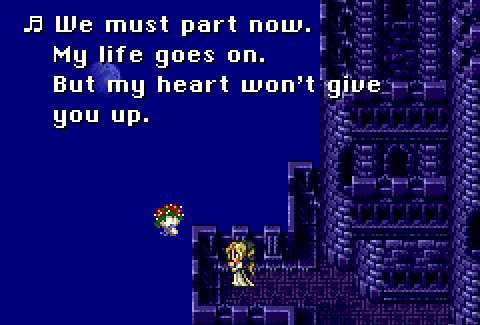
\includegraphics[width=\columnwidth]{./art/mariaanddraco/maria.jpg}\\
%
\vfill
%
\ofbullet{1 ponto por cada linha que o jogador recitou corretamente, até 4 pontos.}
\ofbullet{1 ponto extra, se o jogador realmente tentou cantar os versos.}
\ofbullet{Até 3 pontos a depender de quanto esforço o grupo empregou ao fazer "Maria" realmente se parecer com a Maria.}
\ofbullet{1 ponto se o jogador se lembrar de pegar  as flores, subir as escadas e erguer as flores.}
\ofbullet{O jogador faz um teste de DF~8 para determinar se ele ou ela consegue se portar graciosamente como a Maria. Se for bem sucedido, recompense-o com 2 pontos. A DF pode ser menor se a "Maria" tem qualquer experiência relacionadaa atuação.}
%
\vfill
%
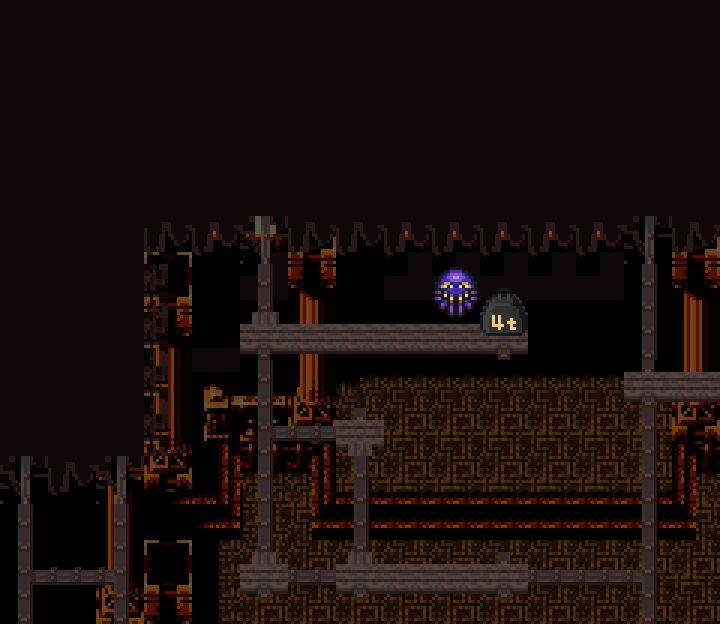
\includegraphics[width=\columnwidth]{./art/mariaanddraco/ultros.png}
%
\vfill
%
Assim que a parte de Maria está terminando no palco, o Empresário e o grupo estão assistindo de seus aposentos.
De repente, ele nota algo na passarela: alguém, ou melhor alguma coisa, está tentando derrubar uma bigorna no palco!
O grupo o reconhece que é um estranho polvo, chamado Ultros, que está por trás desse plano.
Os aventureiros já o encontraram antes e derrotá-lo, então eles querem se vingar por sabotar a opera.
O empresário começa a entrar em pânico e implora para que o grupo frustre os planos de Ultros.
Ele aponta para um quarto ao lado do aposento e os diz para puxarem a alavanca mais a direita que encontrarem.
%
\newpage
%
\ofquote{"Silêncio! Você está na presença do polvo da realeza! Um bandido camponês como você nunca me derrotará!" \\}{Ultros}\\\\
%
Após de saírem de seus acentos, cada personagem tem que fazer um teste de DF~6 para decidir se eles perturbam ou não a audiência. 
Se pelo menos um deles falharem, deduza um ponto da apresentação.
Uma vez no quarto, eles percebem quatro alavancas na parede. A mais à direita abre um caminho até a passarela, as outras tem os seguintes efeitos e puxar cada uma delas reduz um ponto da apresentação da "Maria": alavanca 1, faz o som de um cachorro latindo, a 2, apaga as luzes no salão de opera, a 3, abre um alçapão abaixo de quem a puxou, o que o faz deslizar diretamente até o palco.
Assim que o grupo entrar na passarela, eles verão que Ultros já está para derrubar a bigorna na "Maria". 
À medida que se aproximam, as frágeis tábuas da passarela falham em suportar o peso deles combinados e tanto o grupo quanto Ultros caem no palco.
"Maria" tem que fazer um teste de DF~7 e se falhar, ela fica inconsciente, do contrário, também participa da batalha que iniciará.
Aqueles que caírem, Ultros incluso, recebem 1d de dano, mas podem se levantar de imediato para começar a luta!
%
\vfill
%
\ofmonster{Ultros}{3}{
\includegraphics[width=0.32\columnwidth]{./art/mariaanddraco/ultrosmon.jpg}}
{
	PV: & \hfill 60 & PM: & \hfill 90 \\
	FOR: & \hfill 4 & DEF: & \hfill 2 \\
	MAG: & \hfill 1 & RES: & \hfill 3 \\
	AGI: & \hfill 2 & Tamanho: & \hfill G\\
}
{\accf{Tinta}: 1d Dano, 3u Alcance\hfill \accf{Deix:} 500G\\
\accf{Imune}:\poison\sleep\blind\immobile \hfill \accf{Ataque final, Golpe duplo}
}
{	
	\mspell{Água}{6}{0r}{Único}{4u}{Cause 2d de dano de Água ao alvo.}{\water}
	\mtech{Chuva ácida}{8}{0r}{3u}{Você}{Todos na área sofrem 2d de dano de Água, além disso, fazem um teste de DF~7 ou ficam Envenenados por 1 rodada.
	}{\poison\water}	
	\mtech{Tentáculo}{4}{0r}{2u (frontal)}{Você}{Cause 2d de dano a todos os inimigos na área.}{}	
	\mpassive{Toque cegante}{Cada alvo que rolar abaixo de 6 no teste de evasão contra seus ataques, ficam Cegos por 3 rodadas.}{}		
}
%
\vfill
%
Após o grupo derrotar Ultros, eles escutam uma voz alta exclamando: "Que apresentação!".
De repente, um homem desce no palco usando um arpéu. Ninguém mais, ninguém menos do que o Setzer.
Ele agarra "Maria" rapidamente e ativa o dispositivo mais uma vez para puxar a si até o alojamento, com "Maria" em seus braços.
De lá ele escapa para sua aeronave, a qual o espera sobre o telhado da casa de opera.
O grupo tenta segui-lo, mas eles têm que tomar uma rota mais longa até o telhado.
Assim que chegarem lá, Setzer está prestes a partir.
%
\clearpage
%
\ofquote{"Nada a perder altém de minha vida..."\\}{Setzer}\ofpar
%
%
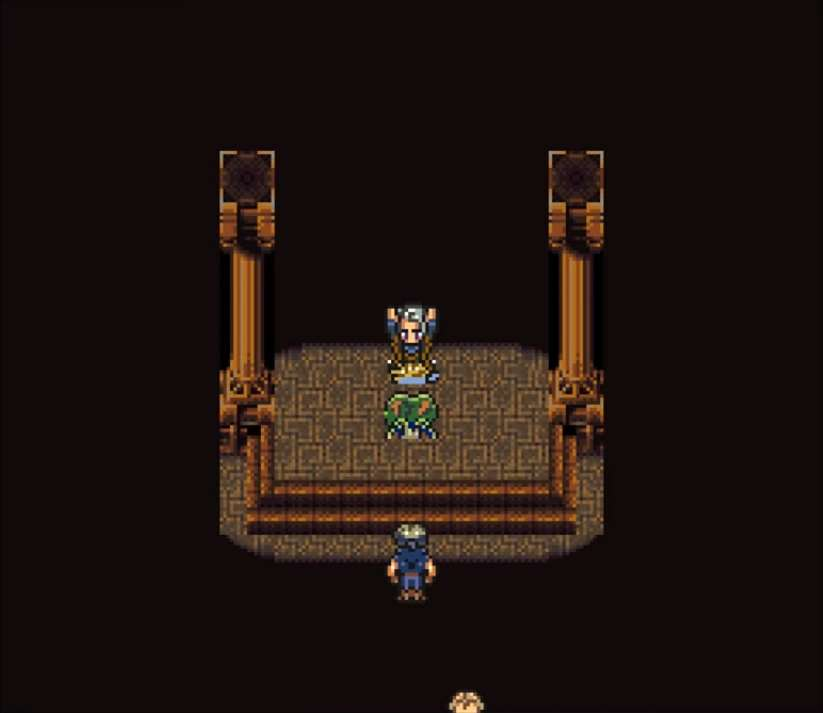
\includegraphics[width=\columnwidth]{./art/mariaanddraco/setzer.jpg} 
%
\ofpar\\
%
Ele prende "Maria" em sua cabine e vai ao deque para ligar o motor.
Se a "Maria" havia ficado inconsciente, ela acordará agora e perceberá que Setzer a raptou.
Se tudo ocorrer de acordo com o plano até aqui, ela deverá ter a corda consigo. Assim sendo, poderá abaixá-la por uma das janelas desse quarto para que o grupo suba por ela. Opcionalmente, você pode pedir a cada membro do grupo que faça um teste de DF~7 para decidir se eles conseguem agarrar e subir por ela com sucesso.
Depois de se distanciar da casa de opera, Setzer retorna à cabine. Após olhar mais de perto a "Maria" e perceber o resto do grupo, ele entende que foi enganado e fica irado.
Como se dará o confronto depende das decisões do grupo. Abaixo seguem algumas ideias de interpretação de Setzer, mas você pode, ou pode ter que, improvisar alguns aspectos dessa parte.
%
\ofpar\\
%
\accf{O grupo tentar resolver o conflito pacificamente:}\\
Setzer normalmente estará aberto a isso ao perceber que está em menor número.
Ele pode ser convencido a deixar o grupo partir e não se manter longe da casa de opera dali então. Assim como, ele também pode ser juntar ao grupo, se oferecerem perspectiva de aventuras empolgantes à frente.
Será muito mais fácil o convencer se o acordo envolver algum tipo de aposta, coisa que ele ama.
Se o grupo tentar trapacear, ele mostrará ainda mais respeito por eles. Entretanto, não aceitará qualquer acordo que envolva ele ser capturado ou entregue às autoridades.
%
\ofpar\\
%
\accf{O grupo tenta matar ou capturar Setzer à força:}\\
Neste caso, as estatísticas de combate de Setzer estão listadas abaixo. Apesar de superado em quantidade, ele não desiste fácil e não hesitará em usar truques baixos para ter a vantagem.
Se o grupo conseguir derrotá-lo, eles podem decidir se querem o deixar vivo ou entregar às autoridades. De qualquer forma, precisarão manobrar e pousar a aeronave.
O jogador que a controlar tem que fazer um teste de DF que pode variar de 6 a 8, a depender da proficiência dele com veículos. Se falhar, a aeronave cai perto de Jidoor e é destruída. Todos os passageiros à bordo sobrevivem, mas sofrem 2d de dano.
%
\vfill
%
\ofmonster{Setzer}{4}{
\includegraphics[width=0.25\columnwidth]{./art/mariaanddraco/setzermon.jpg}}
{
	PV: & \hfill 40 & PM: & \hfill 80 \\
	FOR: & \hfill 2 & DEF: & \hfill 1 \\
	MAG: & \hfill 0 & RES: & \hfill 1 \\
	AGI: & \hfill 4 & Tamanho: & \hfill M\\
}
{
\accf{Cartas}: 2d Dano, 3u Alcance \hfill \accf{Auto-Acelerar}
}
{
	\mtech{Espaços}{8}{0r}{?}{?}{
		Role 1d. Um dos seguintes efeitos ocorrem a depender do resultado:
		em 1 ou 2, a área dentro de 3u de você é preenchida com uma fumaça até o começo de seu próximo turno.
		Todos dentro dela, ficam Cegos, mas também Oscilando.
		em 3 ou 4, teleporte-se para um local à sua escolha dentro de 3u,
		em 5 ou 6, uma explosão causa 2d de dano de Fogo a todos os inimigos dentro de 2u.
	}{}	
	\mtech{Atirar Gil}{4}{0r}{2u}{5u}{Arremesse 100G para causar 2d de dano a todos os inimigos na área.}{}
	\mtech{Sumir}{8}{0r}{Único}{Arma}{Torne-se invisível por 5 rodadas ou até que aja. Enquanto isso, fique Oscilando. Além do mais, se você acertar um ataque enquanto invísivel, será um Acerto crítico automático.}{\blink}	
	\mreaction{Dado fixo}{Sempre que rolar para um teste ou determinar danos, role novamente um dado que resulte em ~1.}{}		
}
%
\vfill
%
Após lidar com Setzer, o grupo pode retornar para a casa de opera e coletar sua recompensa.
O Empresário considerará o contrato cumprido se conseguirem espantar o Setzer. Primeiro, cada membro ganha um \accf{Nível} a mais!
Além disso, também recebem uma recompensa a depender da classificação da atuação de Maria:\\\\
\ofbullet{\accf{1-3 pontos:} apesar de espantar Setzer, a apresentação foi um desastre, deixando a audiência muito insatisfeita. Empresário culpa o grupo de serem descuidades e reduz pela metade a recompensa originalmente oferecida para 500G.}\\\\
\ofbullet{\accf{4-6 points:} apesar dos percalços, a apresentação foi bem. Empresário está satisfeito e entrega ao grupo o montante combinado de 1.000G.}\\\\
\ofbullet{\accf{7-10 points:} o grupo foi capaz de impressionar a audiência com uma apresentação estonteante. Empresário está emocionado e dobra o montante originalmente acordado para 2.000G.}
%
\clearpage